% One-page TableNet architecture diagram with the wheel history encoder: tectonic tablenet_whist_diagram.tex
\documentclass[11pt]{article}
\usepackage[paperwidth=8.5in,paperheight=7.4in,margin=0.5in]{geometry}
\usepackage[T1]{fontenc}
\usepackage{newtxtext,newtxmath}
\usepackage{xcolor,tikz,amsmath}
\usetikzlibrary{positioning,fit,arrows.meta,calc,backgrounds}
\pagestyle{empty}
\definecolor{cblue}{HTML}{2a78d6}
\definecolor{corange}{HTML}{eb6834}
\definecolor{caqua}{HTML}{1baf7a}
\definecolor{cpurple}{HTML}{8c5bd6}
\definecolor{cgray}{HTML}{8a8984}
\tikzset{
  arr/.style={-{Stealth[length=5pt]},draw=black!60,thick},
  box/.style={draw=#1!80!black,fill=#1!10,rounded corners=2pt,inner sep=4pt,align=center},
  box/.default=cgray,
}
\begin{document}
\begin{center}
{\large\bfseries TableNet with a wheel history encoder}\\[2pt]
{\small one network for picks and wheels \quad\textperiodcentered\quad \texttt{train\_tablenet\_joint.py whist\_layers=2}}
\end{center}
\vspace{6pt}
\begin{center}
% TableNet with a wheel history encoder (whist_layers). \input by architecture.tex and tablenet_whist_diagram.tex;
% needs the colours cblue/corange/caqua/cpurple/cgray and the styles box/arr from either preamble.
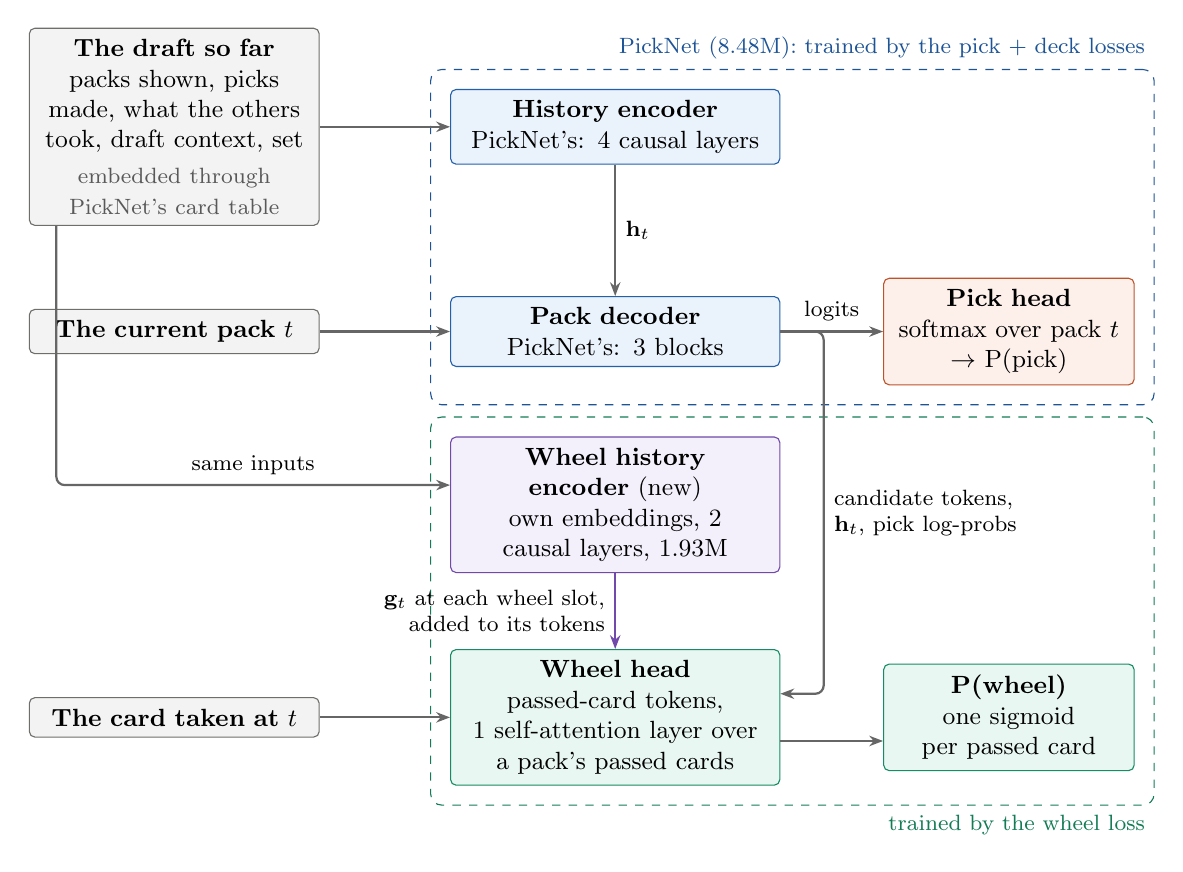
\begin{tikzpicture}[font=\small]
% inputs
\node[box,text width=3.4cm] (data) at (0,0) {\textbf{The draft so far}\\packs shown, picks made, what the others
  took, draft context, set\\[2pt]{\footnotesize\color{black!65}embedded through PickNet's card table}};
\node[box,text width=3.4cm] (pack) at (0,-2.6) {\textbf{The current pack $t$}};
\node[box,text width=3.4cm] (took) at (0,-7.5) {\textbf{The card taken at $t$}};
% PickNet trunk + pick head
\node[box=cblue,text width=3.9cm] (hist) at (5.6,0) {\textbf{History encoder}\\PickNet's: 4 causal layers};
\node[box=cblue,text width=3.9cm] (dec) at (5.6,-2.6) {\textbf{Pack decoder}\\PickNet's: 3 blocks};
\node[box=corange,text width=2.9cm] (pick) at (10.6,-2.6) {\textbf{Pick head}\\softmax over pack $t$\\$\to$ P(pick)};
% wheel side
\node[box=cpurple,text width=3.9cm] (whist) at (5.6,-4.8) {\textbf{Wheel history encoder} (new)\\own embeddings,
  2 causal layers, 1.93M};
\node[box=caqua,text width=3.9cm] (wheel) at (5.6,-7.5) {\textbf{Wheel head}\\passed-card tokens,\\1 self-attention
  layer over a pack's passed cards};
\node[box=caqua,text width=2.9cm] (pw) at (10.6,-7.5) {\textbf{P(wheel)}\\one sigmoid per passed card};
% data flow
\draw[arr] (data) -- (hist);
\draw[arr] (hist) -- node[right,font=\footnotesize]{$\mathbf h_t$} (dec);
\draw[arr] (pack) -- (dec);
\draw[arr] (dec) -- node[above,font=\footnotesize]{logits} (pick);
\draw[arr,rounded corners=3pt] (data.south west) ++(0.35,0) |- ([yshift=0.25cm]whist.west)
  node[pos=0.75,above,font=\footnotesize,align=center]{same inputs};
\draw[arr,draw=cpurple!80!black] (whist) -- node[left,font=\footnotesize,align=right]{$\mathbf g_t$ at each wheel slot,\\added to its tokens} (wheel);
\draw[arr,rounded corners=3pt] (dec.east) -- ++(0.55,0) |- node[pos=0.25,right,font=\footnotesize,align=left]
  {candidate tokens,\\$\mathbf h_t$, pick log-probs} ([yshift=0.3cm]wheel.east);
\draw[arr] (took) -- (wheel);
\draw[arr] ([yshift=-0.3cm]wheel.east) -- ([yshift=-0.3cm]pw.west);
% what each loss trains
\begin{scope}[on background layer]
\node[draw=cblue!70!black,dashed,rounded corners=4pt,inner sep=7pt,fit=(hist)(dec)(pick)] (pn) {};
\node[draw=caqua!70!black,dashed,rounded corners=4pt,inner sep=7pt,fit=(whist)(wheel)(pw)] (wn) {};
\end{scope}
\node[anchor=south east,font=\footnotesize,text=cblue!70!black,align=right] at (pn.north east)
  {PickNet (8.48M): trained by the pick + deck losses};
\node[anchor=north east,font=\footnotesize,text=caqua!70!black,align=right] at (wn.south east)
  {trained by the wheel loss};
\end{tikzpicture}

\end{center}
\vspace{4pt}
{\small
\noindent\textbf{Why the new box.} With one shared history encoder, the pick and wheel losses pull it in opposite
directions, and the wheel task's extra accuracy came only from reshaping it, at a cost to picks. The wheel history
encoder gives the wheel head its own summary of the draft. It reads the same inputs as PickNet's, through PickNet's
card table, so PickNet's history can stay tuned for picks. Its output
projection starts at zero, so training begins exactly at the step-1 wheel head.

\noindent\textbf{Who trains what.} PickNet always trains on the pick and deck losses. The wheel loss trains the wheel
head and the wheel history encoder. How far the wheel loss also reaches into PickNet is set by \texttt{wheel\_block}:
\texttt{all} keeps it out of PickNet entirely (run A); \texttt{hist} keeps it out of PickNet's history encoder only,
so it can still adjust the card table and pack decoder (run B).
}
\end{document}
